\documentclass[12pt]{article}
\usepackage[utf8]{inputenc}
\usepackage[T1]{fontenc}
\usepackage[polish]{babel}
\usepackage{amsmath}
\usepackage{amsthm}
\usepackage[margin=0.7in]{geometry}
\usepackage{dsfont}
\usepackage{mdframed}
\usepackage[many]{tcolorbox}
\usepackage{listings}
\usepackage[bottom]{footmisc}
\usepackage{cite}
\usepackage{float}
\usepackage{graphicx}

\tcbuselibrary{theorems}

\newtcbtheorem[]{theo}{Twierdzenie}%
{
    breakable,
    colback=blue!5,
    colframe=gray!35!black,
    fonttitle=\bfseries,
    before skip=20 pt, 
    after skip=20pt
}{th}

\newtcbtheorem[]{defn}{Definicja}%
{
    breakable,
    colback=blue!5,
    colframe=gray!35!black,
    fonttitle=\bfseries,
    before skip=20 pt, 
    after skip=20pt
}{df}

\newtcbtheorem[]{prog}{Program}%
{
    breakable,
    colback=blue!5,
    colframe=gray!35!black,
    fonttitle=\bfseries,
    before skip=20 pt, 
    after skip=20pt
}{pr}

\lstdefinelanguage{Julia}%
{
    morekeywords={%
        exit,whos,edit,load,is,isa,isequal,typeof,tuple,ntuple,uid,hash,finalizer,convert,promote,%
        subtype,typemin,typemax,realmin,realmax,sizeof,eps,promote_type,method_exists,applicable,%
        invoke,dlopen,dlsym,system,error,throw,assert,new,Inf,Nan,pi,im,begin,while,for,in,return,%
        break,continue,macro,quote,let,if,elseif,else,try,catch,end,bitstype,ccall,do,using,module,%
        import,export,importall,baremodule,immutable,local,global,const,Bool,Int,Int8,Int16,Int32,%
        Int64,Uint,Uint8,Uint16,Uint32,Uint64,Float32,Float64,Complex64,Complex128,Any,Nothing,None,%
        function,type,typealias,abstract%
  },%
  sensitive=true,%
  morecomment=[l]\#,%
  morecomment=[n]{\#=}{=\#},%
  morestring=[s]{"}{"},%
  morestring=[m]{'}{'},%
}[keywords, comments, strings]%

\lstset{%
    language         = Julia,
    basicstyle       = \ttfamily,
    keywordstyle     = \bfseries\color{blue},
    columns          = fullflexible,
    stringstyle      = \color{magenta},
    commentstyle     = \color{gray},
    showstringspaces = false,
    numbers          = left,
    xleftmargin      = 2em
}

\title{\huge Metody wyznaczania liczby $e$}
\date{Analiza Numeryczna (M) - Zadanie P1.4\\ \today}
\author{\Large Jakub Grobelny}

\begin{document}
\begin{titlepage}
\maketitle
\thispagestyle{empty}

\begin{abstract}
    W matematyce istnieje wiele liczb, które są w pewnym sensie interesujące, 
    powtarzają się w różnych kontekstach i gałęziach tejże nauki. Jedną z takich
    liczb jest liczba $e$, zwana też liczbą Eulera lub stałą Napiera. 
    Stała ta jest podstawą logarytmu naturalnego, czyli jedyną taką liczbą, dla 
    której spełnione jest równanie $\ln{e} = 1$.

    Ze względu na częstotliwość występowania liczby $e$ w matematyce, istotne jest
    to, żeby móc ją wystarczająco dokładnie aproksymować. Niniejsze sprawozdanie
    jest podsumowaniem eksperymentu numerycznego polegającego na obliczaniu liczby
    $e$ dwoma sposobami -- korzystając z definicji $e = \lim\limits_{n \to \infty}(1 + \frac{1}{n})^n$ oraz
    z rozwinięcia funkcji $e^x$ w szereg $e^x = \sum_{k=0}^\infty\frac{x^k}{k!}$.
    Porównana została precyzja obu sposobów, oraz ich efektywność.
\end{abstract}

\end{titlepage}

\newpage
\tableofcontents
\newpage

\section{Definicja liczby $e$}


\begin{defn}{Logarytm naturalny}{ln_def}
    Dla $x \in \mathds{R}, x > 0$ logarytm naturalny z $x$ definiujemy następująco:
    \large$$\ln{x} = \int_{1}^{x}\frac{1}{t} dt$$\normalsize
\end{defn}

\begin{defn}{Podstawa logarytmu naturalnego}{e_ln}
    $e$ jest jedyną taką liczbą rzeczywistą, że $\ln{e} = 1$.
\end{defn}

Znając definicję \ref{df:ln_def} możemy sformułować definicję $e$, równoważną definicji
\ref{df:e_ln}.

\begin{defn}{Podstawa logarytmu naturalnego}{}
    $e$ jest jedyną taką liczbą rzeczywistą, że 
    \large$$1 = \int_{1}^{e}\frac{1}{t} dt$$\normalsize
\end{defn}

\subsection{Obliczanie $e$ jako granicy $\lim\limits_{n \to \infty}{(1 + \frac{1}{n})^n}$}

\begin{theo}{}{limit_theorem}
    Liczbę $e$ możemy zdefiniować następująco:
    \large$$e = \lim\limits_{n \to \infty}(1 + \frac{1}{n})^n.$$\normalsize
    \begin{proof}
        $ $
        Niech $t \in [1; 1 + \frac{1}{n}]$.
        Wtedy $$\frac{1}{1 + \frac{1}{n}} \leq \frac{1}{t} \leq 1.$$
        Całkując stronami mamy 
        $$\int_{1}^{1+\frac{1}{n}} {\frac{1}{1+\frac{1}{n}}}\,dt \leq
        \int_{1}^{1+\frac{1}{n}} {\frac{1}{t}}\,dt \leq
        \int_{1}^{1+\frac{1}{n}} {1}\,dt.$$
        Pierwsza całka jest równa $\frac{1}{n+1}$, druga z definicji \ref{df:ln_def} wynosi
        $\ln(1+\frac{1}{n})$, trzecia zaś $\frac{1}{n}$.
        Mamy więc nierówność
        $$\frac{1}{n+1} \leq \ln{(1 + \frac{1}{n})} \leq \frac{1}{n},$$
        którą możemy przekształcić dalej
        $$e^{\frac{1}{n + 1}} \leq 1 + \frac{1}{n} \leq e^{\frac{1}{n}}.$$
        Podnosząc lewą stronę nierówności do potęgi $(n + 1)$ otrzymujemy
        $$e \leq (1 + \frac{1}{n})^{n+1},$$
        podnosząc zaś prawą stronę do potęgi $n$-tej mamy
        $$(1 + \frac{1}{n})^n \leq e.$$
        Z tego wynika, że
        $$(1 + \frac{1}{n})^n \leq e \leq (1 + \frac{1}{n})^{n+1}.$$
        Dzieląc prawą stronę nierówności przez $1 + \frac{1}{n}$ otrzymujemy
        $$\frac{e}{1 + \frac{1}{n}} \leq (1 + \frac{1}{n})^n$$
        co w połączeniu z wcześniejszą nierównością daje nam
        $$\frac{e}{1+\frac{1}{n}} \leq (1 + \frac{1}{n})^n \leq e.$$
        Oczywistym jest, że 
        $\lim\limits_{n \to \infty}{\frac{e}{1 + \frac{1}{n}}} = e$ oraz
        $\lim\limits_{n \to \infty}{e} = e$, więc z twierdzenia o trzech ciągach
        wynika, że
        $$\lim\limits_{n \to \infty}{(1 + \frac{1}{n})^n} = e.$$
    \end{proof}
\end{theo}

Wiedząc, że $e = \lim\limits_{n \to \infty}{(1 + \frac{1}{n})^n}$, wiemy, że 
dla dużych wartości $n$ zachodzi
$$ e \approx (1 + \frac{1}{n})^n. $$
Wykorzystując tę obserwację można sformułować algorytm\footnote{Wszystkie programy w niniejszym sprawozdaniu napisane są w języku Julia w wersji 1.0.1.}, 
który będzie wyznaczał przybliżoną wartość liczby $e$.

\begin{prog}{Funkcja w języku Julia obliczająca $(1 + \frac{1}{n})^n$}{prog1}
    \begin{lstlisting}
function calc_e_lim(n)
    return (1 + 1/n)^n
end
    \end{lstlisting}
\end{prog}

%bibliografia
\subsection{Rozwinięcie $e$ w szereg}

\begin{defn}{Wielomian Taylora \cite{anmat1}}{taylor}
Niech funkcja $f$ ma w punkcie $x_0$ pochodną $k$-tego rzędu, gdzie $k \in \mathds{N}$.
Wielomian
$$f(x_0) + \frac{f'(x_0)}{1!}(x-x_0) + \frac{f''(x_0)}{2!}(x-x_0)^2 + ... + \frac{f^{(k)}(x_0)}{k!}(x-x_0)^k$$
nazywamy wielomianem Taylora rzędu $k$ funkcji $f$ w punkcie $x_0$ i oznaczamy symbolem
$P_k(x)$. Dla $x_0 = 0$ wielomian ten nazywamy wielomianem Maclaurina.
\newline

Wielomian $P_k$ jest jedynym wielomianem stopnia $k$, który spełnia warunki:
$$P_k(x_0) = f(x_0),\, P_k'(x_0) = f'(x_0),\, ...\,, P_k^{(k)}(x_0) = f^{(k)}(x_0)$$
\end{defn}

\begin{theo}{Wzór Taylora z resztą Lagrange'a \cite{anmat1}}{taylor_lagrange}
    Jeżeli funkcja $f$ ma:
    
    1. ciągłą pochodną rzędu $n - 1$ na przedziale $[x_0; x]$,

    2. pochodną właściwą $f^{(n)}$ na przedziale $(x_0; x)$,

    to istnieje punkt $\xi \in (x_0; x)$ taki, że
    $$f(x) = \sum_{k = 0}^{n - 1}\frac{f^{(k)}(x_0)}{k!}(x-x_0)^k + \frac{f^{(n)}(\xi)}{n!}(x-x_0)^n.$$

    Powyższe twierdzenie jest prawdziwe także dla przedziału $[x; x_0]$, wtedy $\xi\in(x;x_0)$.

    Równość występującą w tezie twierdzenia nazywamy wzorem Taylora, a wyrażenie
    $$R_n(x) \overset{def}{=} \frac{f^{(n)}(\xi)}{n!}(x-x_0)^n$$
    $n$-tą resztą Lagrange'a. Resztę Lagrange'a można także zapisać w postaci
    $$R_n(x) \overset{def}{=} \frac{f^{(n)}(x_0 + \Theta\Delta x)}{n!}(\Delta x)^n,$$
    gdzie $0 < \Theta < 1$ oraz $\Delta x = x - x_0$.

    Dla $x_0 = 0$ wzór Taylora przyjmuje postać
    $$f(x) = \sum_{k = 0}^{n-1}\frac{f^{(k)}(0)}{k!}x^k + \frac{f^{(n)}(\xi)}{n!}x^n,$$
    gdzie $\xi \in (0; x)$ dla $x > 0$ lub $\xi \in (x; 0)$ dla $x < 0$. Równość tę
    nazywamy wzorem Maclaurina.
    \newline
    
    Dla $n \to \infty$ mamy
    $$f(x) = \sum_{k = 0}^{\infty}\frac{f^{(k)}(0)}{k!}x^k$$

    \begin{proof}
        Dowód w \cite{anmat1}, na stronie 125.
    \end{proof}
\end{theo}

Znając powyższe twierdzenie można zapisać funkcję $f(x) = e^x$ w postaci szeregu przy
użyciu wzoru Maclaurina.
Najpierw można zaobserwować, że \large$$\forall{n \in \mathds{N}}\,\,( f^{(n)}(x) = e^x).$$\normalsize
Powyższa obserwacja umożliwa rozwinięcie $f(x)$ w szereg
$$f(x) = \sum_{k = 0}^{\infty}\frac{f^{(k)}(0)}{k!}x^k 
= \sum_{k = 0}^{\infty}\frac{e^0}{k!}x^k
= \sum_{k = 0}^{\infty}\frac{x^k}{k!}.$$
$e = e^1 = f(1)$, więc ostatecznie można wyznaczyć następujący wzór na $e$ podstawiając $x = 1$:

\large
\begin{align}
e = \sum_{k = 0}^{\infty}\frac{1}{k!}. \label{series}
\end{align}\normalsize

\begin{prog}{Funkcja w języku Julia obliczająca sumę $n$ wyrazów szeregu (\ref{series})}{prog2}
    \begin{lstlisting}
function calc_e_series(n)
    fact = 1.0 # kolejne wartosci k!
    sum = fact # suma szeregu
    # pomijane jest obliczanie pierwszego wyrazu rownego 1/0!
    for k in 1:n
        fact *= k
        sum += 1/fact
    end
    return sum
end
    \end{lstlisting}
\end{prog}

\section{Opis eksperymentu}

Obliczenia zostały wykonane w języku Julia (wersja 1.0.1)
przy użyciu 256-bitowej arytmetyki (256 bitów przeznaczonych na reprezentację mantysy).

Programy \ref{pr:prog1} i \ref{pr:prog2} zostały uruchomione dla różnych wartości $n$,
a następnie została porównana precyzja, z jaką przybliżają liczbę $e$ poprzez porównanie wyniku
do wbudowanej stałej \texttt{MathConstants.e}. 

Obliczona została liczba cyfr znaczących
każdego przybliżenia przy użyciu wzoru
\large$$\lfloor - log_{10}(\delta_e) \rfloor,$$\normalsize gdzie 
\large$$\delta_e = |\frac{\Delta e}{e}|$$\normalsize
i 
\large$$\Delta e = e - \widetilde{e},$$\normalsize
gdzie $\widetilde{e}$ oznacza otrzymane przybliżenie $e$.

\subsection{Oszacowanie szybkości zbieżności obu programów}

Przed wykonaniem obliczeń można spróbować oszacować ile iteracji każdej
metody jest potrzebne, aby uzyskać maksymalnie dokładne przybliżenie $e$.

\begin{defn}{Wykładnik zbieżności ciągu}{convergence_rate}
    Niech ciąg $a_n$ będzie zbieżny do $g$. Jeżeli istnieją takie,
    liczby $p, C \in \mathds{R},\,\, C > 0$, że,
    \large$$\lim\limits_{n \to \infty}{\frac{|a_{n+1} - g|}{|a_n - g|^p}} = C,$$\normalsize
    to $p$ nazywamy \textbf{wykładnikiem zbieżności} ciągu $a_n$, a $C$ -- \textbf{stałą asymptotyczną błędu}.
    Dla $p = 1$ oraz $0 < C < 1$ zbieżność jest \textbf{liniowa}, dla $p = 2$ ,
    \textbf{kwadratowa}, dla $p = 3$ -- \textbf{sześcienna}.
    
    Dla $p = 1$ i $C = 1$ zbieżność jest \textbf{podliniowa}.

    Jeżeli ciąg $a_n$ zbiega do $g$ podliniowo, oraz
    $$\lim\limits_{n \to \infty}{\frac{|a_{n+2} - a_{n+1}|}{|a_{n+1} - a_n|}} = 1,$$

    to mówimy, że ciąg $a_n$ zbiega \textbf{logarytmicznie} do $g$.
\end{defn}

Można obliczyć wykładnik zbieżności ciągu $(1+\frac{1}{n})^n$ korzystając z definicji
\ref{df:convergence_rate}. Okazuje się, że ten \textbf{ciąg jest zbieżny do $e$ logarytmicznie},
więc kolejne przbliżenia polepszają się nieznacznie. \newline

W przypadku drugiej metody oszacowanie potrzebnej wartości $n$, która zagwarantuje
maksymalnie dużą precyzję wyniku, okazuje się być prostszym zadaniem.

\begin{defn}{Precyzja arytmetyki}{precision}
    Precyzją arytmetyki danego komputera nazywamy liczbę
    \large$$ u = \frac{1}{2}\, 2^{-t},$$\normalsize
    gdzie $t \in \mathds{N}$ jest liczbą bitów przeznaczonych na mantysę.
\end{defn}

Można zauważyć, że korzystając ze wzoru (\ref{series}) od pewnego momentu kolejne
składniki sumy będą mniejsze niż precyzja arytmetyki. Oznacza to, że 
od tego momentu przybliżenie nie będzie się już zmieniać, gdyż $1 + u = 1$.

Przyjęto, że liczba bitów przeznaczonych na mantysę wynosi 256, mamy więc
$$u = \frac{1}{2}\,2^{-256}$$
$$u = 2^{-257}$$

Dla ostatniego znaczącego składnika sumy szeregu ze wzoru (\ref{series}) spełniona 
musi więc być nierówność
$$\frac{1}{k!} \leq 2^{-257}.$$
$$k! \geq 2^{257}.$$
Rozwiązaniem jest $k \geq 57$. Można spodziewać się, że liczba iteracji
większa niż $k$ nie polepszy już otrzymanego przybliżenia $e$, jeżeli do jego
obliczenia użyty zostanie program \ref{pr:prog2}. Nie oznacza to jednak, że reszta
szeregu (\ref{series}) jest mniejsza niż używana precyzja arytmetyki. 
W zaproponowanym algorytmie wyrazy są jednak sumowane po kolei, w taki sposób, że
każdy kolejny jest dodawany do dotychczasowej sumy, przez co można przypuszczać, że
powyższa obserwacja będzie miała odzwierciedlenie w praktyce.

\section{Wyniki obliczeń i ich analiza}

\begin{figure}[H]
    \centering
    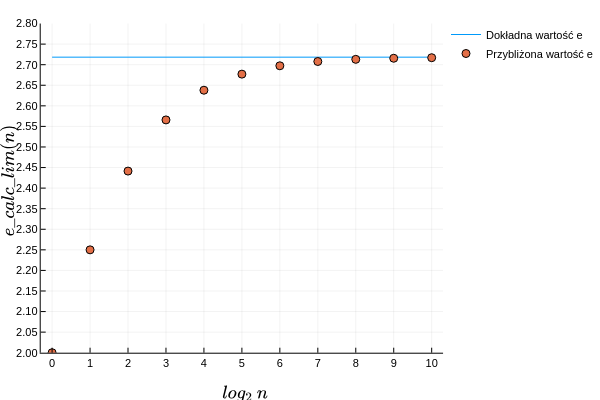
\includegraphics[scale=0.75]{plot1.png}
\caption{Wykres przedstawiający wyniki programu \ref{pr:prog1} dla $n = 2^0, 2^1, ..., 2^{10}$}
\label{figure:fig1}
\end{figure}

\begin{table}[H]
\centering
\begin{tabular}{|c|c|}
    \hline
    \large $n$ & \large Liczba cyfr znaczących przybliżenia $e$\normalsize\\
    \hline
    $2^1$    & 0  \\ \hline
    $2^2$    & 0  \\ \hline
    $2^3$    & 1  \\ \hline
    $2^4$    & 1  \\ \hline
    $2^5$    & 1  \\ \hline
    $2^6$    & 2  \\ \hline
    $2^7$    & 2  \\ \hline
    $2^8$    & 2  \\ \hline
    $2^9$    & 3  \\ \hline
    $2^{10}$ & 3  \\ \hline
    \vdots  & \vdots \\ \hline
    $2^{252}$& 76 \\ \hline
\end{tabular}
\caption{Wyniku programu \ref{pr:prog1} dla wybranych wartości $n$}
\label{table:prog1}
\end{table}

\begin{table}[H]
\centering
\begin{tabular}{|c|c|}
    \hline
    \large$n$ & \large Liczba cyfr znaczących przybliżenia $e$\normalsize\\
    \hline
    1   &  0  \\ \hline
    2   &  1  \\ \hline
    3   &  1  \\ \hline
    4   &  2  \\ \hline
    5   &  3  \\ \hline
    6   &  4  \\ \hline
    7   &  4  \\ \hline
    8   &  5  \\ \hline
    9   &  6  \\ \hline
    10  &  7  \\ \hline
    11  &  9  \\ \hline
    21  &  21 \\ \hline
    31  &  35 \\ \hline
    41  &  51 \\ \hline
    51  &  58 \\ \hline
    55  &  75 \\ \hline
    56  &  76 \\ \hline
    57  &  76 \\ \hline
    58  &  76 \\ \hline
    61  &  76 \\ \hline
    71  &  76 \\ \hline
    81  &  76 \\ \hline
    91  &  76 \\ \hline
\end{tabular}
\caption{Wyniki programu \ref{pr:prog2} dla wybranych wartości $n$}
\label{table:prog2}
\end{table}

\begin{figure}[H]
    \centering
    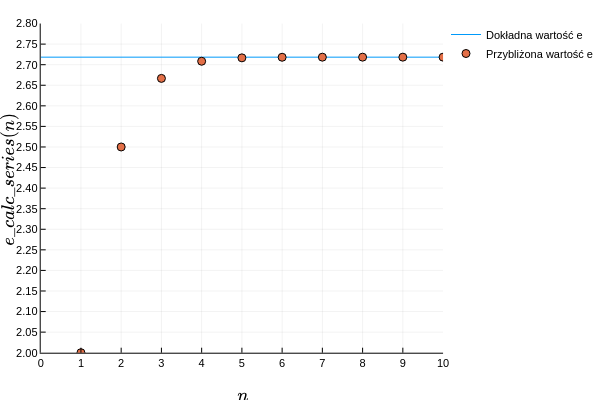
\includegraphics[scale=0.75]{plot2.png}
\caption{Wykres przedstawiający wyniki programu \ref{pr:prog2} dla $n = 1, 2, ..., 10$}
\label{figure:fig2}
\end{figure}

Jak widać w tablicy \ref{table:prog1}, otrzymane 
przybliżenie $e$ przy użyciu programu \ref{pr:prog1} jest bardzo niedokładne 
nawet dla $n = 2^{10}$. Wyniki są zgodne z oczekiwaniami, gdyż ciąg $(1+\frac{1}{n})^n$ 
zbiega do $e$ logarytmicznie. W tablicy \ref{table:prog1} wyszczególniony został 
wynik dla $n=2^{252}$, gdyż jest to pierwsza wartość $n$, dla której uzyskana 
została (w przybliżeniu) taka sama precyzja, jaką udało się uzyskać przy wykorzystaniu 
programu \ref{pr:prog2}. Przy założeniu, że operacja potęgowania w Julii wykonuje 
się w czasie $O(log_2\,b)$, gdzie $b$ jest to wykładnik potęgi, można oszacować
złożoność programu \ref{pr:prog1} na $O(log_2\,n)$. Widać wtedy dysproporcje pomiędzy
dwoma algorytmami. Pierwszy z nich potrzebuje $252$ iteracje aby osiągnąć wynik,
który drugi zwraca już przy $56$ iteracjach (program \ref{pr:prog2} oczywiście ma
złożoność $O(n)$).

Tablica \ref{table:prog2} potwierdza również wcześniejsze przypuszczenia, że
liczba iteracji większa bądź równa $57$ nie polepszy już dokładności wyniku przy
zastosowaniu 256-bitowej precyzji.

Uzyskane wyniki pokazują, że obliczanie $e$ z definicji
\large$$e = \lim\limits_{n \to \infty}{(1+\frac{1}{n})^n}$$\normalsize
jest gorszym sposobem numerycznego obliczania tej stałej niż przy
wykorzystaniu wzoru
\large$$e = \sum_{k=0}^{\infty}\frac{1}{k!}.$$\normalsize

\begin{figure}[H]
    \centering
    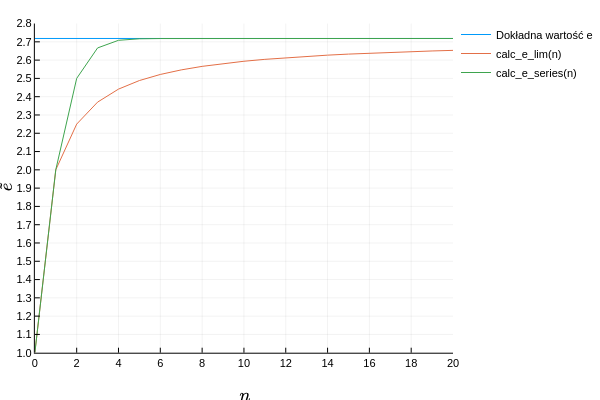
\includegraphics[scale=0.75]{plot3.png}
\caption{Wykres porównujący wyniki obu programów w jednakowej skali}
\label{figure:fig3}
\end{figure}

Dane przedstawione na rysunkach \ref{figure:fig1} i \ref{figure:fig2} mogą być nieco
mylące, ze względu na różną skalę osi $x$, więc zostały one przedstawione również
na rysunku \ref{figure:fig3}, który pozwala na lepszą analizę otrzymanych wyników.
Widać, że wykres dla funkcji \texttt{calc\_e\_lim} jest o wiele bardziej spłaszczony, niż
ten dla funkcji \texttt{calc\_e\_series}.

Zakładając, że \texttt{calc\_e\_lim} ma złożoność $O(log_2\,n)$ można przedstawić
wyniki tak jak na rysunku \ref{figure:fig4}, gdzie na osi $x$ znajduje się przybliżona
liczba iteracji algorytmu (w przypadku programu \ref{pr:prog1} iteracje rozumiemy
jako liczbę kroków potrzebnych do podniesienia wyrażenia $(1+\frac{1}{n})$ do potęgi $n$).

\begin{figure}[H]
    \centering
    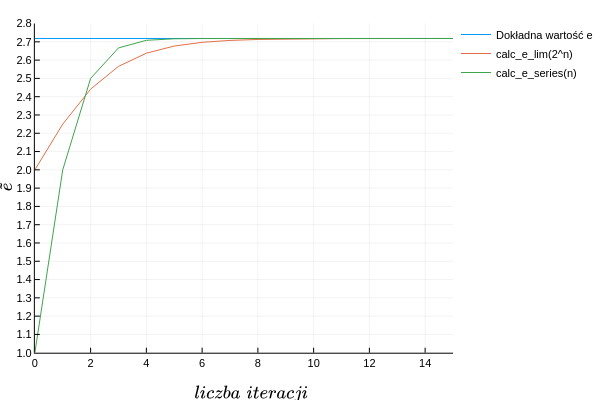
\includegraphics[scale=0.75]{plot4.png}
\caption{Wykres porównujący wyniki obu programów dla danej liczby iteracji}
\label{figure:fig4}
\end{figure}

Widać, że nawet przy takim spojrzeniu na otrzymane rezultaty, funkcja 
\texttt{calc\_e\_series} dalej jest zauważalnie lepsza niż funkcja \texttt{calc\_e\_lim}.


\addcontentsline{toc}{section}{Bibliografia}
\bibliography{bibliografia}{}
\bibliographystyle{plain}

\end{document}
